\chapter{Fine and Hyperfine Structure of Hydrogen}
\label{ch:fine}

% ============================================================
\section{Spin in the Hydrogen Atom}
% ============================================================

So far the electron in hydrogen was described by $|n,\ell,m\rangle$, eigenstates of $\{\hat{H}_{\text{Coul}},\hat{\vect{L}}^2,\hat{L}_z\}$. Including the spins of the electron and proton, the Hilbert space is $\mathcal{H} = \mathcal{H}_{\mathbb{R}^3}\otimes\mathcal{H}^{(e)}_{1/2}\otimes\mathcal{H}^{(p)}_{1/2}$, with CSCO $\{\hat{H}_{\text{Coul}},\hat{\vect{L}}^2,\hat{L}_z,\hat{\vect{S}}_e^2,\hat{S}_{ez},\hat{\vect{S}}_p^2,\hat{S}_{pz}\}$. The Coulomb interaction is spin-independent, so this tensor product would be trivial. But there are small additional effects:
\[
    \hat{H} = \hat{H}_{\text{Coul}} + \underbrace{\alpha\,\hat{\vect{S}}_e\cdot\hat{\vect{L}}}_{\text{spin--orbit}} + \underbrace{\beta\,\hat{\vect{S}}_e\cdot\hat{\vect{S}}_p}_{\text{hyperfine}} .
\]
Now $[\hat{H},\hat{L}_z] = -i\alpha\hbar\epsilon_{ij3}\hat{S}_{ei}\hat{L}_j\neq0$, and likewise $\hat{S}_{ez}$ and $\hat{S}_{pz}$ no longer commute with $\hat{H}$. The total $\hat{\vect{J}} = \hat{\vect{L}} + \hat{\vect{S}}_e + \hat{\vect{S}}_p$ does: $[\hat{H},\hat{J}_z] = [\hat{H},\hat{\vect{J}}^2] = 0$.

The set $\{\hat{H},\hat{\vect{L}}^2,\hat{\vect{S}}_e^2,\hat{\vect{S}}_p^2,\hat{\vect{J}}^2,\hat{J}_z\}$ is not yet complete: $\ell\otimes\frac12\otimes\frac12 = (\ell+1)\oplus\ell\oplus\ell\oplus(\ell-1)$ contains two $j = \ell$ multiplets. One more operator is needed to separate them. Partial sums such as $\hat{\vect{J}}_{ep}^2 = (\hat{\vect{S}}_e+\hat{\vect{S}}_p)^2$ would do mathematically, but none commutes with $\hat{H}$. Only the combination $\hat{J}_{\alpha\beta}^2 = \frac\alpha2\hat{\vect{J}}_{eL}^2 + \frac\beta2\hat{\vect{J}}_{ep}^2$, which equals $\Delta\hat{H}$ plus Casimirs, does, completing the CSCO.

% ============================================================
\section{First-Order Perturbation Theory}
% ============================================================

\begin{theorem}[Feynman--Hellmann]
If $\hat{H}(\lambda)|\Psi(\lambda)\rangle = E(\lambda)|\Psi(\lambda)\rangle$ with $|\Psi(\lambda)\rangle$ normalized, then
\[
    \frac{dE}{d\lambda} = \Bigl\langle\Psi(\lambda)\Bigl|\frac{d\hat{H}}{d\lambda}\Bigr|\Psi(\lambda)\Bigr\rangle .
\]
\end{theorem}
\begin{proof}
Differentiate $E = \langle\Psi|\hat{H}|\Psi\rangle$; the terms from differentiating the states give $E\,\frac{d}{d\lambda}\langle\Psi|\Psi\rangle = 0$.
\end{proof}

\begin{formula}[First-order energy shift]
For $\hat{H}(\lambda) = \hat{H}_0 + \lambda\hat{H}_1$ with $\lambda\ll1$, the shift of the eigenvalue of an $\hat{H}_0$ eigenstate $|\Psi_0\rangle$ is
\[
    \Delta E = \langle\Psi_0|\Delta\hat{H}|\Psi_0\rangle + O(\lambda^2),
\]
the expectation value of the perturbation in the unperturbed state. ($|\Psi_0\rangle$ is not an eigenstate of $\hat{H}$; this simplest form of perturbation theory says nothing about the new states.)
\end{formula}

% ============================================================
\section{Spin--Orbit Coupling}
% ============================================================

In the electron's rest frame the proton is a moving charge, producing a field $\vect{B}\approx-\frac1c\lvect{v}\times\vect{E}$. With the radial field $\vect{E} = \frac{1}{4\pi\varepsilon_0}\frac{e}{r^2}\rhat$ this is $\vect{B} = \frac{1}{4\pi\varepsilon_0}\frac{e}{m_ecr^3}\vect{L}$, which couples to the electron's moment. The electron's frame is not inertial, and the relativistic correction (Thomas precession) effectively replaces $g_e\approx2$ by $g_e-1\approx1$:

\begin{formula}[Spin--orbit Hamiltonian]
\[
    \Delta\hat{H}_{SL} = \frac{e^2}{8\pi\varepsilon_0m_e^2c^2}\frac{1}{r^3}\,\hat{\vect{S}}_e\cdot\hat{\vect{L}} .
\]
\end{formula}

The radial expectation value is $\langle n,\ell,m|r^{-3}|n,\ell,m\rangle = [n^3a^3\ell(\ell+1)(\ell+\frac12)]^{-1}$ for $\ell\neq0$. (It can be derived from the radial equation via the Feynman--Hellmann theorem below: treating $\ell$ as a continuous parameter in the effective potential gives $\langle r^{-2}\rangle = [n^3a^2(\ell+\frac12)]^{-1}$, and the expectation value of the radial equation's derivative relates $\langle r^{-3}\rangle$ to $\langle r^{-2}\rangle$ by $\langle r^{-3}\rangle = \langle r^{-2}\rangle/a\ell(\ell+1)$.) (For $\ell = 0$ this naive calculation fails, since the electron sits on the proton; there the dominant correction is the Darwin term.) $\hat{L}_z$ and $\hat{S}_{ez}$ do not commute with $\Delta\hat{H}_{SL}$, but with $\hat{\vect{J}} = \hat{\vect{L}} + \hat{\vect{S}}_e$,
\[
    \hat{\vect{L}}\cdot\hat{\vect{S}}_e = \frac12\bigl(\hat{\vect{J}}^2 - \hat{\vect{L}}^2 - \hat{\vect{S}}_e^2\bigr),
\]
which is diagonal in the coupled basis $|n,\ell,s,j,m_j\rangle$:
\[
    \hat{\vect{L}}\cdot\hat{\vect{S}}_e|n,\ell,s,j,m_j\rangle = \frac{\hbar^2}{2}\Bigl[j(j+1) - \ell(\ell+1) - \frac34\Bigr]|n,\ell,s,j,m_j\rangle .
\]

\begin{example}[The $\ell = 1$ level]
$1\otimes\frac12 = \frac32\oplus\frac12$: six states. In the coupled basis,
\[
    |\tfrac32,\tfrac32\rangle = |1,1\rangle|{\uparrow}\rangle,
    \qquad
    |\tfrac32,\tfrac12\rangle = \sqrt{\tfrac23}|1,0\rangle|{\uparrow}\rangle + \sqrt{\tfrac13}|1,1\rangle|{\downarrow}\rangle,
    \qquad
    |\tfrac12,\tfrac12\rangle = -\sqrt{\tfrac13}|1,0\rangle|{\uparrow}\rangle + \sqrt{\tfrac23}|1,1\rangle|{\downarrow}\rangle,
\]
and similarly for negative $m_j$. Then $\langle\hat{\vect{L}}\cdot\hat{\vect{S}}_e\rangle = \frac{\hbar^2}{2}(+1)$ for the four $j = \frac32$ states and $\frac{\hbar^2}{2}(-2)$ for the two $j = \frac12$ states: the six-fold level splits into a quartet and a doublet.
\end{example}

\begin{example}[Size of the spin--orbit splitting]
For $n = 2$, $\ell = 1$, using $\langle r^{-3}\rangle = 1/24a^3$ and $\langle\hat{\vect{L}}\cdot\hat{\vect{S}}_e\rangle$ differing by $\frac32\hbar^2$ between $j = \frac32$ and $j = \frac12$,
\[
    \Delta E = \frac{e^2}{8\pi\varepsilon_0m_e^2c^2}\cdot\frac{1}{24a^3}\cdot\frac32\hbar^2 = \frac{\alpha^4m_ec^2}{32}\approx4.5\times10^{-5}\ \text{eV},
\]
using $a = \hbar/\alpha m_ec$ and $e^2/4\pi\varepsilon_0 = \alpha\hbar c$. Relative to the Bohr energy $\frac18\alpha^2m_ec^2$ this is of order $\alpha^2\approx5\times10^{-5}$, the origin of the name ``fine'' structure.
\end{example}

\begin{formula}[Fine-structure energy]
Combining the spin--orbit term with the relativistic kinetic correction $-\hat{p}^4/8m^3c^2$ (and the Darwin term for $\ell = 0$), the total fine-structure shift depends only on $n$ and $j$:
\[
    E_{nj} = -\frac{\text{Ry}}{n^2}\Bigl[1 + \frac{\alpha^2}{n^2}\Bigl(\frac{n}{j+\frac12} - \frac34\Bigr)\Bigr].
\]
So $2s_{1/2}$ and $2p_{1/2}$ remain degenerate, and $2p_{3/2}$ lies $\frac{\alpha^2}{16}\text{Ry}\approx4.5\times10^{-5}$\,eV above them. The small splitting of $2s_{1/2}$ from $2p_{1/2}$ that is actually observed is the Lamb shift, a QED effect.
\end{formula}

\begin{figure}[ht]
\centering
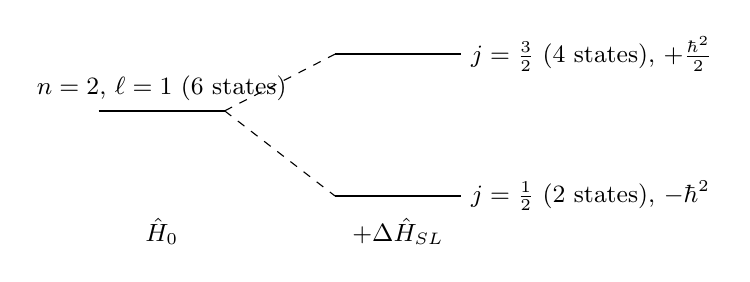
\begin{tikzpicture}[yscale=0.9]
  \draw[thick] (0,2) -- (1.6,2) node[midway,above]{\small $n=2$, $\ell=1$ (6 states)};
  \draw[thick] (3,2.8) -- (4.6,2.8) node[right]{\small $j=\frac32$ (4 states), $+\frac{\hbar^2}{2}$};
  \draw[thick] (3,0.8) -- (4.6,0.8) node[right]{\small $j=\frac12$ (2 states), $-\hbar^2$};
  \draw[dashed] (1.6,2) -- (3,2.8); \draw[dashed] (1.6,2) -- (3,0.8);
  \node at (0.8,0.3) {\small $\hat{H}_0$}; \node at (3.8,0.3) {\small $+\Delta\hat{H}_{SL}$};
\end{tikzpicture}
\caption{Spin--orbit splitting of an $\ell = 1$ level, labelled by $\langle\hat{\vect{L}}\cdot\hat{\vect{S}}_e\rangle$.}
\end{figure}

% ============================================================
\section{Hyperfine Structure}
% ============================================================

The proton is also spin-$\frac12$, with magnetic moment $\bm{\mu}_p = +\frac{g_pe}{2m_p}\hat{\vect{S}}_p$, $g_p\approx5.6$ (far from 2, because of the proton's internal structure), compared with $\bm{\mu}_e = -\frac{g_ee}{2m_e}\hat{\vect{S}}_e$. Its dipole field, including the contact term at the origin (from the vector potential $\vect{A} = -\bm{\mu}_p\times\grad\frac1r$ and $\laplacian\frac1r = -4\pi\delta^3(\lvect{r})$), is
\[
    \vect{B}_p(\lvect{r}) = \frac{1}{c^2r^3}\bigl[3(\bm{\mu}_p\cdot\rhat)\rhat - \bm{\mu}_p\bigr] + \frac{8\pi}{3c^2}\bm{\mu}_p\,\delta^3(\lvect{r}),
\]
giving
\[
    \Delta\hat{H}_{HF} = -\bm{\mu}_e\cdot\vect{B}_p = Q\,\hat{S}_{ei}\hat{S}_{pj}X_{ij}(\lvect{r}),
    \qquad
    X_{ij} = \frac{3\hat{r}_i\hat{r}_j - \delta_{ij}}{r^3} + \frac{8\pi}{3}\delta_{ij}\delta^3(\lvect{r}),
    \qquad
    Q = \frac{g_pe^2}{2m_em_pc^2}.
\]
In the ground state the first term in $X_{ij}$ integrates to zero over angles, leaving the contact term with $|\psi_{100}(0)|^2 = 1/\pi a^3$:
\[
    \langle\Delta\hat{H}_{HF}\rangle_{100} = \frac{8Q}{3a^3}\hat{\vect{S}}_e\cdot\hat{\vect{S}}_p = \underbrace{\frac43g_p\frac{m_e}{m_p}m_ec^2\alpha^4}_{\Delta E_{HF}\,\approx\,5.9\times10^{-6}\,\text{eV}}\frac{\hat{\vect{S}}_e\cdot\hat{\vect{S}}_p}{\hbar^2},
\]
still an operator on the spins. With $\hat{\vect{S}}_e\cdot\hat{\vect{S}}_p = \frac12(\hat{\vect{J}}^2 - \frac32\hbar^2)$ and $\frac12\otimes\frac12 = 1\oplus0$, the triplet shifts up by $\frac14\Delta E_{HF}$ and the singlet down by $\frac34\Delta E_{HF}$. Explicitly, $\hat{\vect{J}}^2 = 2\hbar^2$ in the triplet and $0$ in the singlet, so $\hat{\vect{S}}_e\cdot\hat{\vect{S}}_p/\hbar^2 = \frac12(2-\frac32) = \frac14$ or $\frac12(0-\frac32) = -\frac34$. The splitting is $\Delta E_{HF}$, a weighted average of zero over the four states ($3\times\frac14 - \frac34 = 0$), as must hold for any traceless perturbation.

\begin{figure}[ht]
\centering
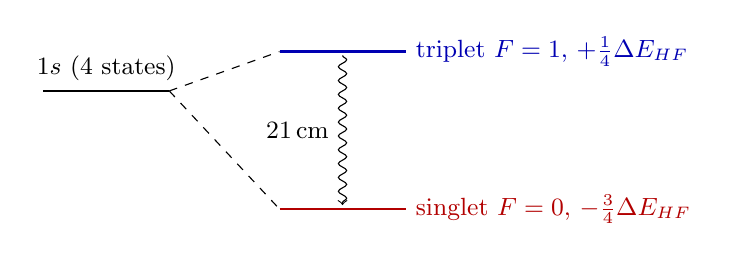
\begin{tikzpicture}[yscale=1]
  \draw[thick] (0,1) -- (1.6,1) node[midway,above]{\small $1s$ (4 states)};
  \draw[thick,blue!70!black] (3,1.5) -- (4.6,1.5) node[right]{\small triplet $F=1$, $+\frac14\Delta E_{HF}$};
  \draw[thick,red!70!black] (3,-0.5) -- (4.6,-0.5) node[right]{\small singlet $F=0$, $-\frac34\Delta E_{HF}$};
  \draw[dashed] (1.6,1) -- (3,1.5); \draw[dashed] (1.6,1) -- (3,-0.5);
  \draw[->,decorate,decoration={snake,amplitude=1.5pt,segment length=5pt}] (3.8,1.45) -- (3.8,-0.45);
  \node[left] at (3.75,0.5) {\small 21\,cm};
\end{tikzpicture}
\caption{Hyperfine splitting of the hydrogen ground state. The transition between the levels emits the 21\,cm line.}
\end{figure}

\begin{fact}[The hydrogen 21\,cm line]
The hyperfine transition from the triplet to the singlet emits a photon of $\lambda = hc/\Delta E_{HF} = 21.1$\,cm ($\nu = 1420$\,MHz). The lifetime is $\sim10^7$\,years, but the cosmic microwave background ($k_BT\approx2\times10^{-4}$\,eV $\gg\Delta E_{HF}$) keeps re-exciting hydrogen throughout the galaxy. The 21\,cm radiation passes through dust, was first seen in 1951, and revealed the spiral structure of the Milky Way. Its Doppler shifts in other galaxies show their outer parts rotating too fast for the visible matter: evidence for dark matter.
\end{fact}

\begin{example}[Muonic hydrogen and the proton radius]
A muon ($m_\mu\approx207m_e$) bound to a proton has a Bohr radius $\sim200$ times smaller, $\sim10^{-12}$\,m, so it is far more sensitive to the proton's finite charge radius $r_{\text{ch}} = |\langle\hat{r}^2\rangle_{\text{proton}}|^{1/2}$. Measured from hyperfine and Lamb-shift transitions, electronic hydrogen gave $r_{\text{ch}} = 0.8775(51)$\,fm and muonic hydrogen $0.84087(39)$\,fm, a $7\sigma$ discrepancy (the ``proton radius puzzle''). Later electronic measurements have moved toward the muonic value.
\end{example}

\begin{fact}[Hierarchy of hydrogen energy scales]
\begin{align*}
    &\text{Bohr energy} && \sim\alpha^2m_ec^2,\\
    &\text{fine structure (spin--orbit, relativistic)} && \sim\alpha^4m_ec^2 &&(\text{relative }10^{-4}),\\
    &\text{Lamb shift (QED)} && \sim\alpha^5m_ec^2 &&(\text{relative }10^{-6}),\\
    &\text{hyperfine splitting} && \sim\alpha^4m_ec^2\,m_e/m_p &&(\text{relative }10^{-7}).
\end{align*}
\end{fact}

% ============================================================
\section{The Zeeman Effect}
% ============================================================

In an external field $\vect{B} = B\khat$, the electron's orbital and spin moments couple as
\[
    \hat{H}_Z = -(\bm{\mu}_L + \bm{\mu}_S)\cdot\vect{B} = \frac{\mu_B B}{\hbar}\bigl(\hat{L}_z + 2\hat{S}_z\bigr),
    \qquad
    \mu_B = \frac{e\hbar}{2m_e}\approx5.79\times10^{-5}\ \text{eV/T},
\]
using $g_e\approx2$ for spin. How to treat it depends on its size relative to the fine structure.

\paragraph{Strong field (Paschen--Back).} If $\hat{H}_Z$ dominates the spin--orbit coupling, the good quantum numbers are $m_\ell$ and $m_s$, and to first order
\[
    E = E_n + \mu_BB(m_\ell + 2m_s).
\]

\paragraph{Weak field.} If $\hat{H}_Z$ is small compared with the fine-structure splitting, the good states are the coupled $|n,\ell,j,m_j\rangle$, and the shift is $\langle\hat{H}_Z\rangle = \frac{\mu_BB}{\hbar}\langle\hat{J}_z + \hat{S}_z\rangle$. $\langle\hat{J}_z\rangle = \hbar m_j$, but $\hat{S}_z$ is not diagonal. Within a multiplet of fixed $j$, any vector operator's expectation value is proportional to that of $\hat{\vect{J}}$ (its component along $\hat{\vect{J}}$ is all that survives the averaging over the precession of $\hat{\vect{S}}$ about $\hat{\vect{J}}$):
\[
    \langle\hat{\vect{S}}\rangle = \frac{\langle\hat{\vect{S}}\cdot\hat{\vect{J}}\rangle}{\hbar^2j(j+1)}\langle\hat{\vect{J}}\rangle,
    \qquad
    \hat{\vect{S}}\cdot\hat{\vect{J}} = \frac12\bigl(\hat{\vect{J}}^2 + \hat{\vect{S}}^2 - \hat{\vect{L}}^2\bigr).
\]

\begin{formula}[Weak-field Zeeman effect]
\[
    \Delta E = g_J\mu_BBm_j,
    \qquad
    g_J = 1 + \frac{j(j+1) + s(s+1) - \ell(\ell+1)}{2j(j+1)},
\]
the Land\'e $g$-factor. Each $j$ level splits into $2j+1$ equally spaced sublevels.
\end{formula}

\begin{example}[Hydrogen $n = 2$]
For $2p_{3/2}$ ($\ell = 1$, $j = \frac32$), $g_J = 1 + \frac{15/4+3/4-2}{15/2} = \frac43$; for $2p_{1/2}$, $g_J = \frac23$; for $2s_{1/2}$, $g_J = 2$. So in a weak field the $2p_{1/2}$ doublet splits by $\frac23\mu_BB$ per unit $m_j$ and $2p_{3/2}$ by $\frac43\mu_BB$: the ``anomalous'' Zeeman effect, which was historically a key clue to electron spin.
\end{example}

\begin{figure}[ht]
\centering
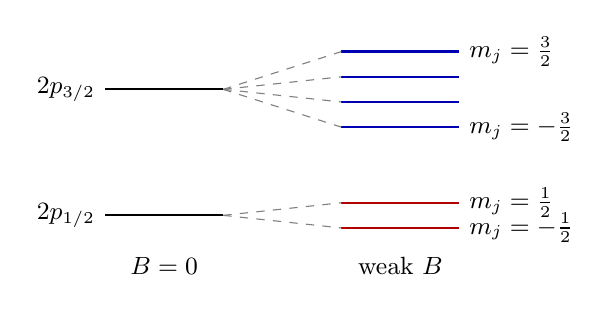
\begin{tikzpicture}[yscale=0.8]
  \draw[thick] (0,2) -- (1.5,2) node[left,pos=0]{\small $2p_{3/2}$};
  \draw[thick] (0,0) -- (1.5,0) node[left,pos=0]{\small $2p_{1/2}$};
  \foreach \m/\y in {3/2.6,1/2.2,-1/1.8,-3/1.4} {\draw[thick,blue!70!black] (3,\y) -- (4.5,\y); \draw[dashed,gray] (1.5,2) -- (3,\y);}
  \node[right] at (4.5,2.6) {\small $m_j=\frac32$}; \node[right] at (4.5,1.4) {\small $m_j=-\frac32$};
  \foreach \y in {0.2,-0.2} {\draw[thick,red!70!black] (3,\y) -- (4.5,\y); \draw[dashed,gray] (1.5,0) -- (3,\y);}
  \node[right] at (4.5,0.2) {\small $m_j=\frac12$}; \node[right] at (4.5,-0.2) {\small $m_j=-\frac12$};
  \node at (0.75,-0.8) {\small $B=0$}; \node at (3.75,-0.8) {\small weak $B$};
\end{tikzpicture}
\caption{Weak-field Zeeman splitting of the $n = 2$, $\ell = 1$ fine-structure levels. The spacings are $g_J\mu_BB$, with $g_J = \frac43$ and $\frac23$.}
\end{figure}

\begin{fact}[Key results of this chapter]
\leavevmode
\begin{itemize}
\item First-order shift: $\Delta E = \langle\Psi_0|\Delta\hat{H}|\Psi_0\rangle$ (Feynman--Hellmann).
\item Spin--orbit coupling $\propto\hat{\vect{L}}\cdot\hat{\vect{S}} = \frac12(\hat{\vect{J}}^2-\hat{\vect{L}}^2-\hat{\vect{S}}^2)$ is diagonal in $|j,m_j\rangle$; fine structure $\sim\alpha^4m_ec^2$.
\item Hyperfine coupling $\hat{\vect{S}}_e\cdot\hat{\vect{S}}_p$ splits the ground state: the 21\,cm line.
\item Zeeman effect: $\Delta E = g_J\mu_BBm_j$ in weak fields.
\end{itemize}
\end{fact}
